\documentclass[12pt,a4paper]{scrartcl}

\usepackage[utf8]{inputenc}
\usepackage[T1]{fontenc}
\usepackage[british,UKenglish,USenglish,american]{babel}

\usepackage[pdftex]{graphicx}
\usepackage{latexsym}
\usepackage{amsmath,amssymb,amsthm}
\allowdisplaybreaks
\usepackage{dsfont}
\usepackage{pifont}
\usepackage{nicefrac}
\usepackage{textcomp}
\usepackage{enumitem}
\usepackage{lmodern}
\usepackage{bbm}

% Abstand obere Blattkante zur Kopfzeile ist 2.54cm - 15mm
\setlength{\topmargin}{-15mm}	   
                  
%\numberwithin{equation}{section} 
\numberwithin{equation}{subsection}

\newcommand{\C}{\mathbb{C}} % komplexe
\newcommand{\R}{\mathbb{R}} % reelle
\newcommand{\Q}{\mathbb{Q}} % rationale
\newcommand{\Z}{\mathbb{Z}} % ganze
\newcommand{\N}{\mathbb{N}} % natuerliche
\newcommand{\PP}{\mathbb{P}} % Probability
\newcommand{\E}{\mathcal{E}} % big Epsilon
\newcommand{\K}{\mathcal{K}}
\newcommand{\1}{\mathbbm{1}}
\newcommand{\G}{\mathcal{G}}
\newcommand{\GG}{\mathfrak{G}}

\numberwithin{equation}{section}

\theoremstyle{definition}
\newtheorem{example}{Example}[subsection]
\newtheorem{theorem}{Theorem}[subsection]
\newtheorem{corollary}{Corollary}[subsection]
\newtheorem{lemma}{Lemma}[subsection]
\newtheorem{definition}{Definition}[subsection]
\newtheorem{proposition}{Proposition}[subsection]
\newtheorem{algorithm}{Algorithm}[subsection]
\newtheorem{prop}{Proposition}[subsection]
\newtheorem{remark}{Remark}[subsection]
\newtheorem{pro}{Proof}
\newtheorem{comment}{Comment}[subsection]


\begin{document}
	\pagestyle{empty}

\begin{titlepage}

	
\includegraphics[scale=0.45]{kit-logo.jpg} 
    \vspace*{2cm} 
\begin{center} \large 
    
   Trash
\end{center}
\end{titlepage}

\newpage

\newpage
\phantom \\
\newpage

\tableofcontents %Inhaltsverzeichnis

 	\pagestyle{headings}

\setcounter{page}{1}

\newpage
\section{Einleitung}
External DLA beschreibt einen stochastischen Prozess, welcher zumindest in ähnlicher Form in natürlichen Prozessen beobachtbar ist. Er ähnelt zum Beispiel der fraktalen Gestalt eines sich kreisförmig ausbreitenden Risses einer Glasscheibe, oder eines Risses eines Kristallfluids wie in LCD Displays in alten Autoradios (siehe Fotos). Er kann auch in Schneeflocken oder in elektrostatischen Anhaftungen an Metallen beobachtet werden. Die Formalisierung solcher Prozesse ist sehr aktuell und die sehr konstruktive Definition erlaubten bisher nur mühsame Folgerungen über Struktur und Verhalten des Prozesses. Wir werden uns Modelle auf $\mathbb{Z}^2$, sowie auf anderen Graphen, darunter auch fraktale Graphen, anschauen, und außerdem versuchen, eine Approximation der bisherigen Definition zu finden, die grundsätzlich handlicher ist und auf einfachere Weise zu Erkenntnissen führt. Wir werden außerdem diese Arbeit mit einigen Python Simulationen begleiten. Der Code ist frei verfügbar auf Github. \\
\\

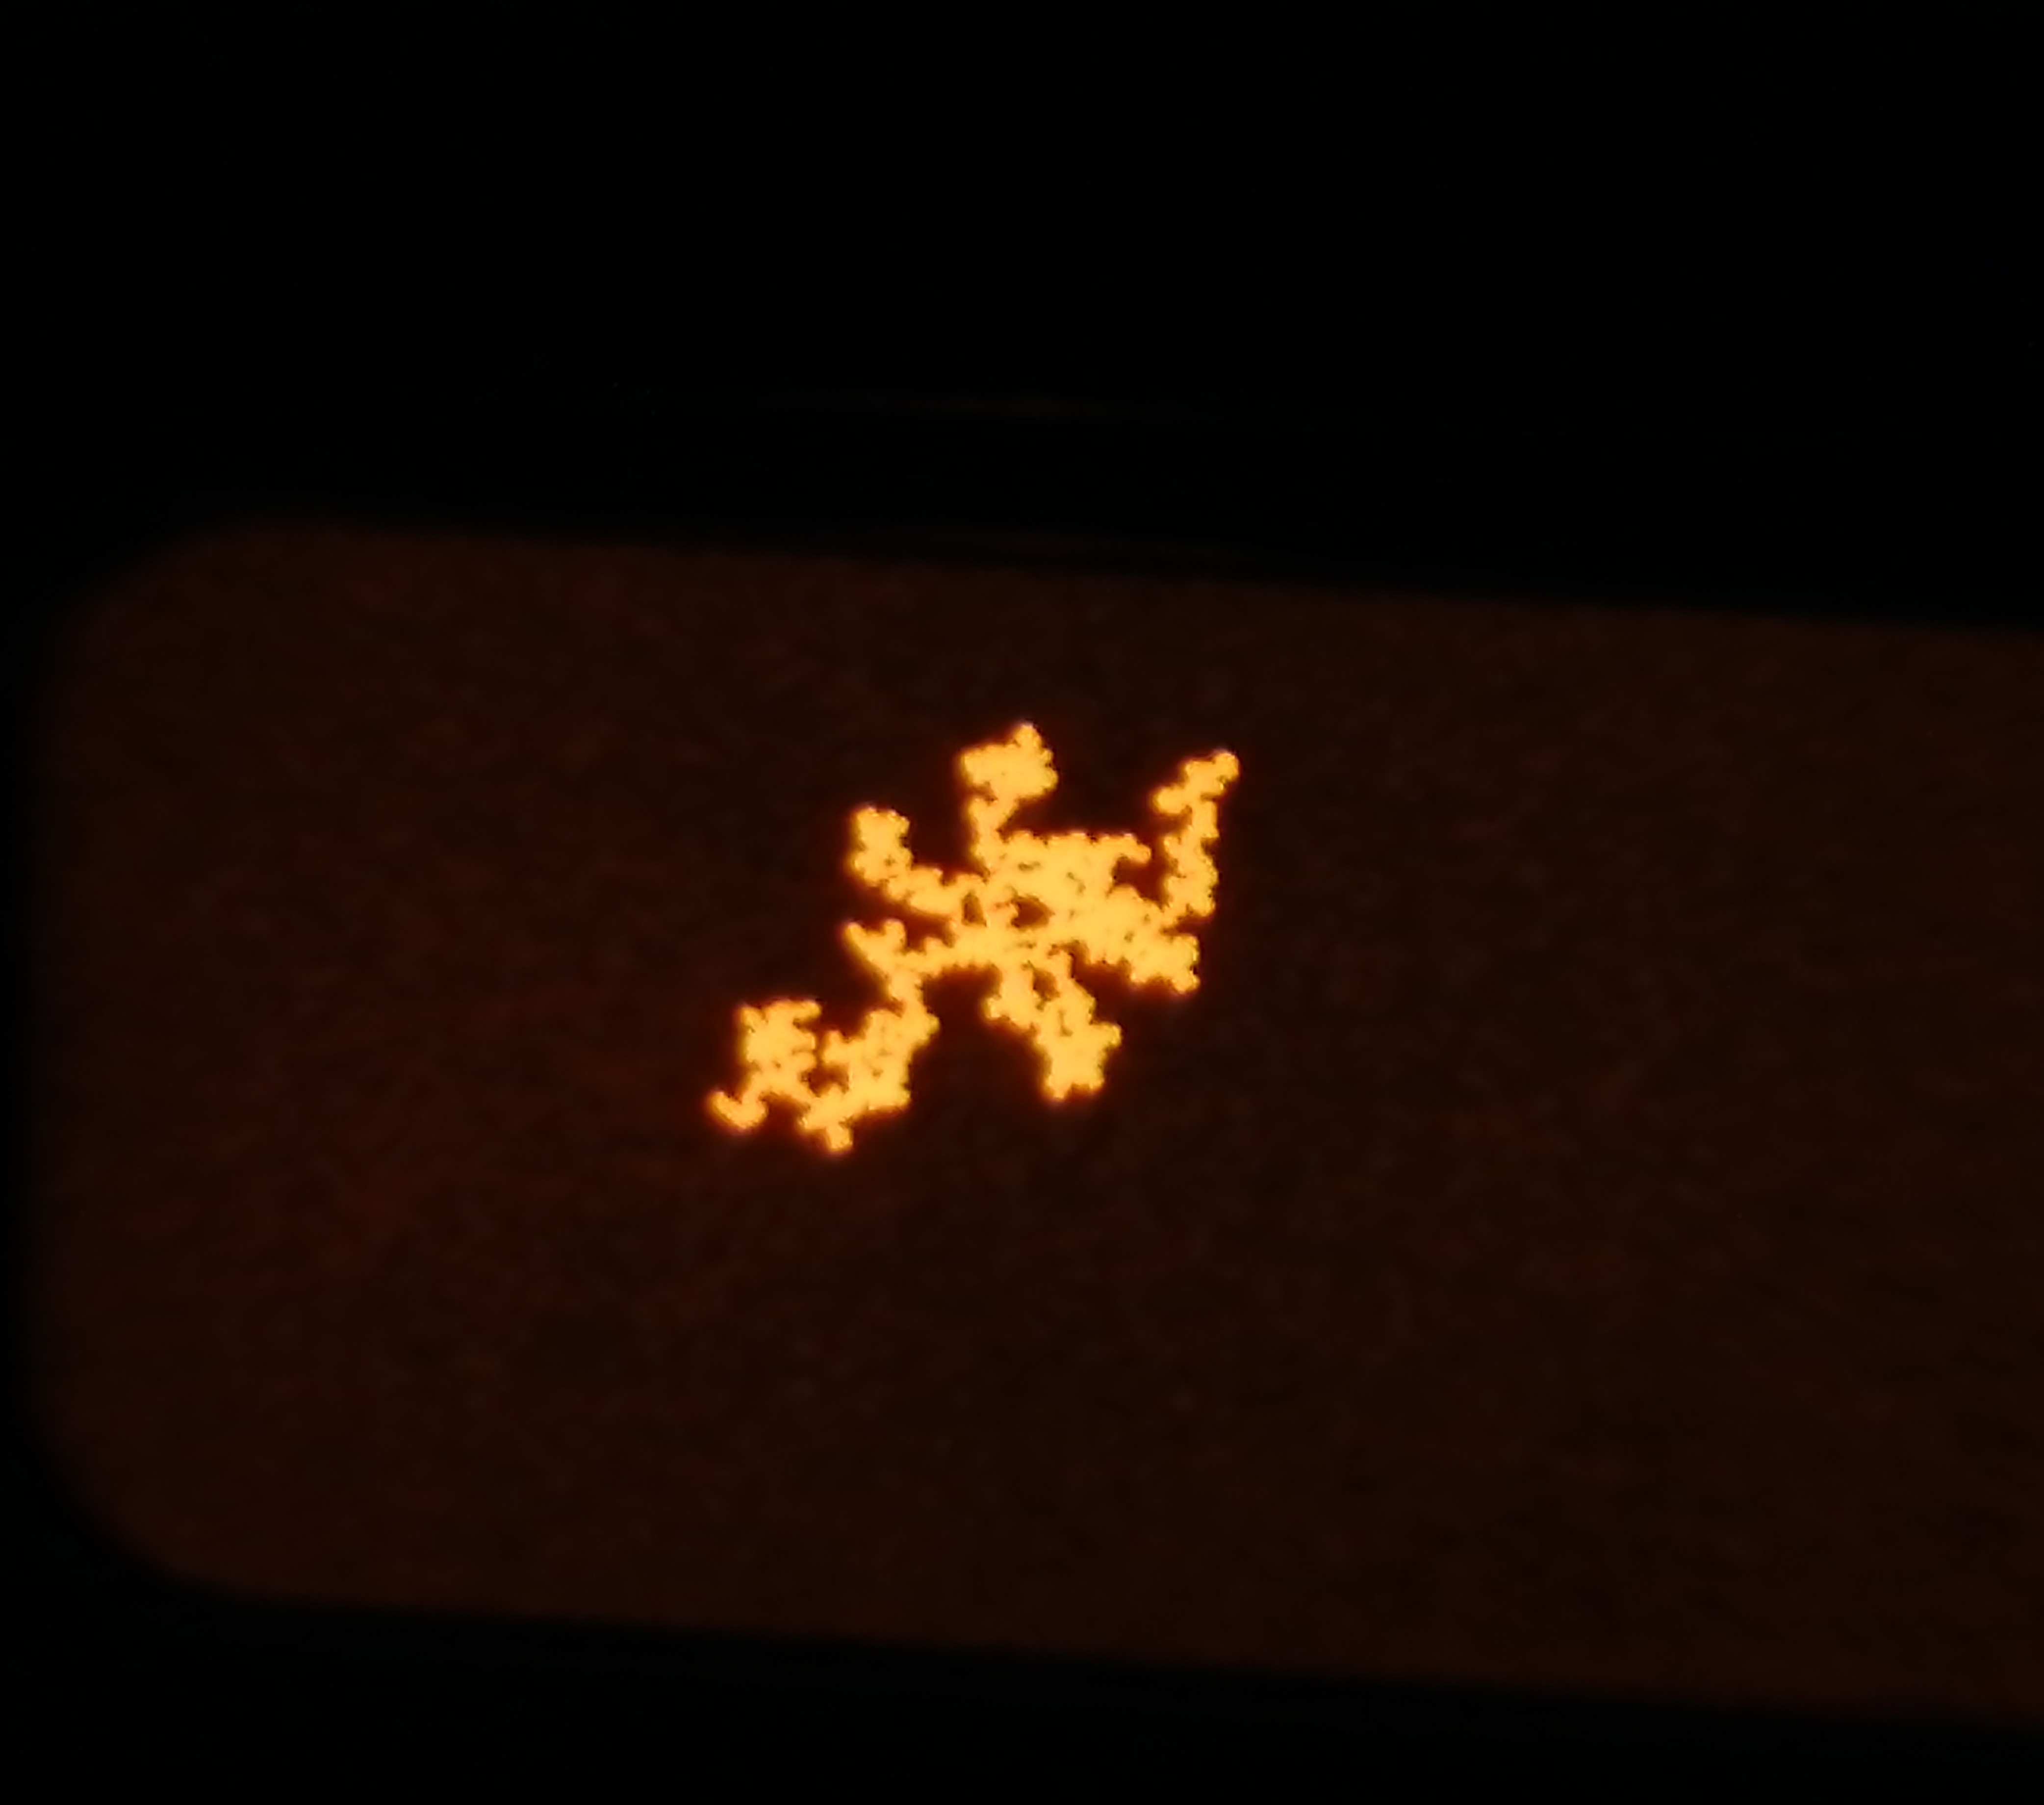
\includegraphics[scale=0.04]{display.jpg} 
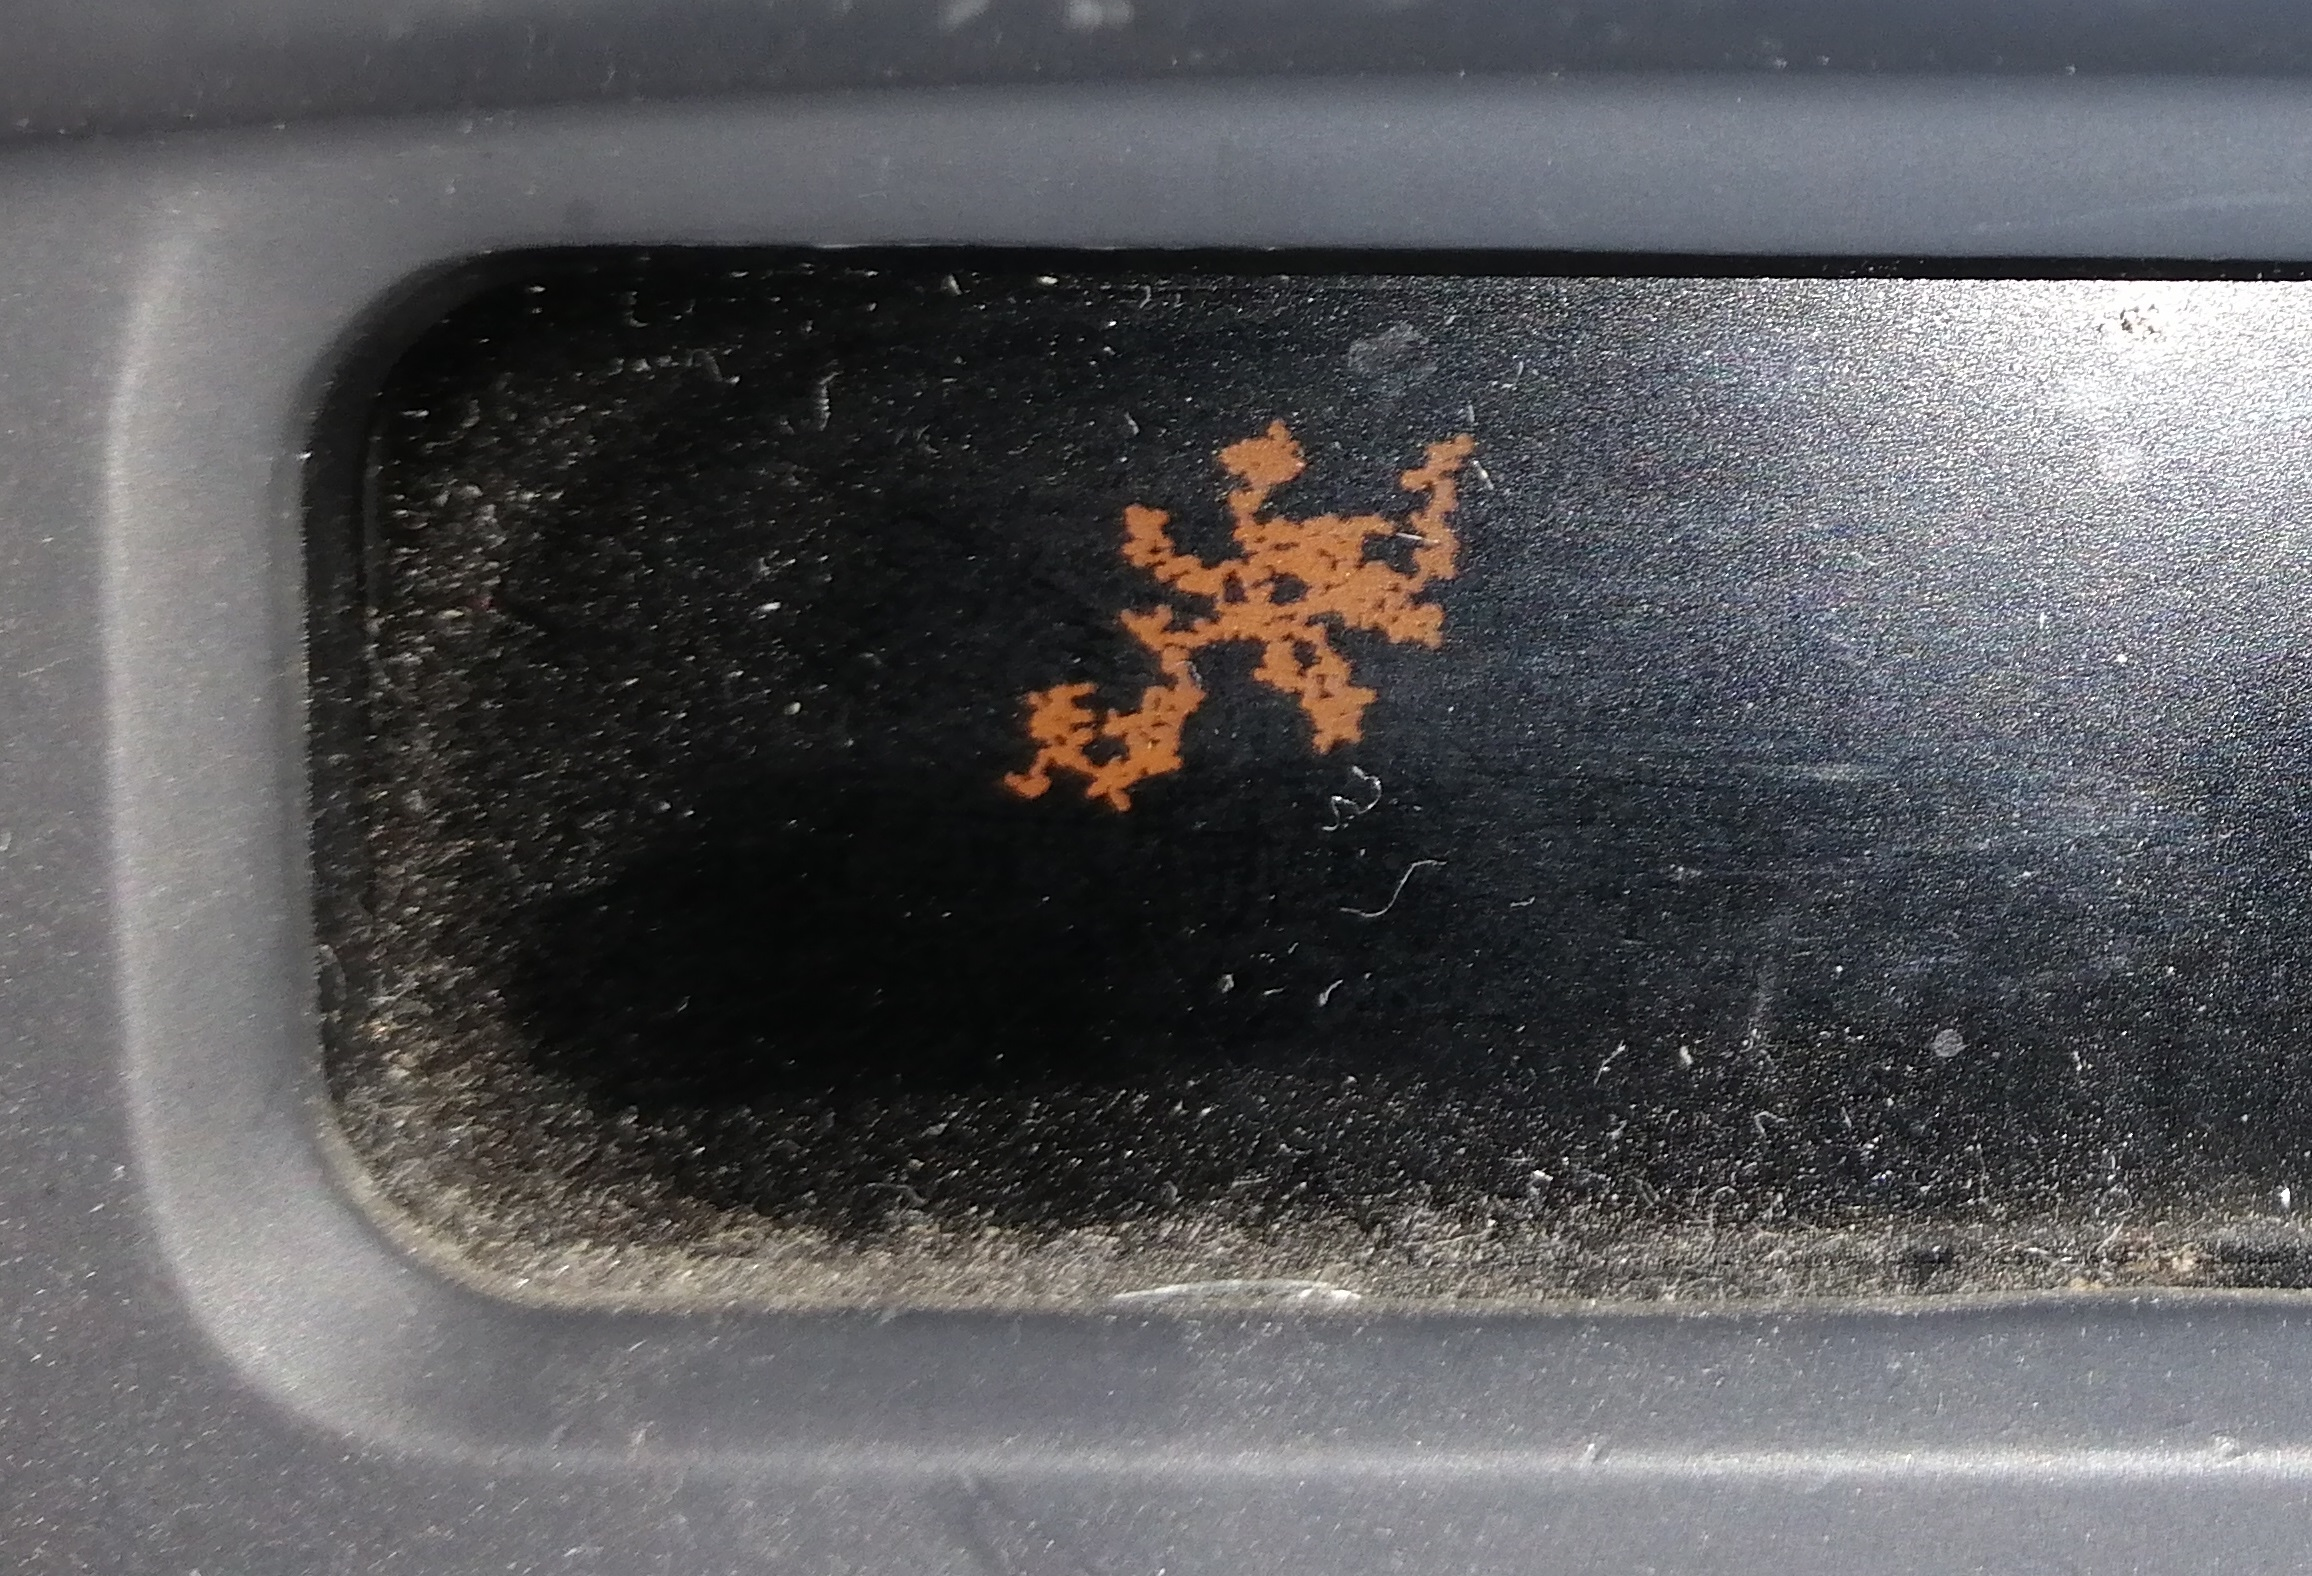
\includegraphics[scale=0.091]{display2.jpg} 

\newpage
\section{harmonic measure}
For the following we are interested in letting start the random walk "from infinity". Thus we are looking for someting like $\lim_{|x|\to\infty} h_A(x,y)$ for $y\in A$. This is solved the following way. Define the $\mathit{escape\ probability}$ from $A$  
\begin{flalign*}
e_A(x) := \1\{x\in A\}\PP(T_A^+=\infty), \quad x\in \Z^2
\end{flalign*}
and the $\mathit{capacity}$ of $A$
\begin{flalign*}
cap(A) := \sum_{x\in \Z^2} e_A(x). 
\end{flalign*}
Note that this sum is finite since $A$ is finite. Now we can define the $\mathit{harmonic\ measure}$ (from infinity) of $A$ as
\begin{flalign*}
h_A(x) := \frac{e_A(x)}{cap(A)}, \quad x\in \Z^2.
\end{flalign*}
The idea here is to use the symmetry of random walks and to not look the probability of coming from infinity to hit $A$, but actually starting in $A$ and stating the probability to escape $A$, which means to never hit $A$ again and therefore necessarily move away to infinity. We finally define the harmonic measure $h=(h_A)_{A\in \mathcal{P}_f}$.

\begin{lemma}
	Does something like $\lim_{|x|\to\infty} h_A(x,y)$ exist and is it equal to $h_A(y)$ for all $y\in A$?
\end{lemma}

\newpage
\section{A naive attempt}

We will look closer at the thought of the last Remark and find a reason, why this way of choosing a random line intersecting $K_0\in\K^2$ is maybe not the best idea. 

\begin{definition}
	Let $\gamma \sim \mathcal{U}([0,\pi))$ and for $\alpha \in [0,\pi)$ define $y_\alpha \sim \mathcal{U}(M_\alpha(K_0))$ where 
	\begin{align*}
		M_\alpha(K):= \begin{cases}
		\{h\in \mathbb{R}\ |\ L_{\tbinom{0}{h}, \tbinom{1}{0}} \cap K \neq \emptyset\},\quad \text{ if } \alpha = 0\\
		\{h\in \mathbb{R}\ |\ L_{\tbinom{h}{0}, \tbinom{cos(\alpha)}{sin(\alpha)}} \cap K \neq \emptyset\},\quad \text{ if } \alpha\in (0,\pi).
		\end{cases} 
	\end{align*}
	For $K\in \K^2$ define 

	\begin{flalign*}
		\nu_{K_0}(K) := \int_{[0,\pi)} \mathbb{P}_{y_\alpha}(M_\alpha(K\cap K_0)) \mathbb{P}_\gamma(d\alpha).
	\end{flalign*}
	Interpretation: $\nu_{K_0}(K)$ is the probability that a random line which intersects with $K_0$ also intersects with $K_0 \cap K$. \\
	Conjecture: $\nu_{K_0}(K) = \frac{\mu_1(K\cap K_0)}{\mu_1(K_0)}$ for $K,K_0\in \K^2$ ($\mu_1$  Gradenmaß).
\end{definition}

\begin{remark}
	Note that $	M_\alpha(K) \in\K^1$ for all $K\in \K^2$ and $\alpha\in [0,\pi)$ (Proof). Proof rotation symmetry.
\end{remark}

\begin{example}
	Let $0<r<R$ and $K_0 := B_R$ and analogously $K:=B_r$. Note that $K,K_0\in \K^2$ and $K\subset K_0$. Then by trigonometry we get 
	\begin{flalign*}
		M_\alpha(K_0) = \begin{cases}
			[-R,R],\quad \text{ if } \alpha=0,\\
			[-\frac{R}{sin(\alpha)}, \frac{R}{sin(\alpha)}],\quad \text{ if } \alpha\in (0,\pi)
		\end{cases}
	\end{flalign*} 
	and analogously $M_\alpha(K)$. Finally we get
	\begin{flalign*}
		\nu_{K_0}(K) &= \int_{[0,\pi)} \PP_{y_\alpha}(M_\alpha(K\cap \K_0)) \mathbb{P}_\gamma(d\alpha)\\
					&= \int_{[0,\pi)} \frac{\lambda(M_\alpha(K))}{\lambda(M_\alpha(K_0))} \frac{d\alpha}{\lambda([0,\pi))}\\
					&= \frac{1}{\pi} \int_{[0,\pi)} \frac{2r}{2R} d\alpha
					= \frac{1}{\pi} \frac{r}{R} \int_{[0,\pi)} 1 d\alpha
					= \frac{r}{R}
	\end{flalign*}
	This result makes sense considering the symmetries of the balls $B_r$ and $B_R$ and the relation of their diameters. 
\end{example}

\begin{example}
	Let $0<r\leq \frac{R}{\sqrt{2}}$, $K_0 := B_R$ as above and $K:= [-r,r]^2$. Note that $K,K_0\in \K^2$ and $K\subset K_0$. We get 
	\begin{flalign*}
		M_\alpha(K) = \begin{cases}
		[-r,r],\quad \text{ if } \alpha\in \{0,\frac{\pi}{2}\},\\
		[-r(1+\frac{1}{tan(\alpha)}),\ r(1+\frac{1}{tan(\alpha)})],\quad \text{ if } \alpha\in (0,\pi)\setminus \{\frac{\pi}{2}\}
		\end{cases}
	\end{flalign*}
	and finally 
	\begin{flalign*}
		\nu_{K_0}(K) &= \int_{[0,\pi)} \PP_{y_\alpha}(M_\alpha(K)) \mathbb{P}_\gamma(d\alpha)\\
		&= \frac{1}{\pi} \int_{(0,\pi)\setminus \{\frac{\pi}{2}\}} \frac{r}{R} (sin(\alpha) + cos(\alpha)) d\alpha\\
		&= \frac{r}{R\pi} [-cos(\alpha) + sin(\alpha)]^\pi_0 
		= \frac{r}{R\pi} (1 + 1) = \frac{2r}{R\pi}
	\end{flalign*}	
\end{example}

\begin{example}
	Let $K_0 := B_R$ and $K:=[-r,r]$ for some $0<r\leq R$. Note $K_0,K\in \K^2$ and $K\subset K_0$. Then 
	\begin{flalign*}
		M_\alpha(K) = \begin{cases}
			\{0\},\quad \alpha = 0,\\
			[-r,r],\quad \alpha\in (0,\pi).
		\end{cases}
	\end{flalign*}
	and finally
	\begin{flalign*}
		\nu_{K_0}(K) = \frac{1}{\pi} \int_{(0,\pi)} \frac{r}{R} sin(\alpha) d\alpha = \frac{2r}{R\pi}.
	\end{flalign*}
\end{example}

\begin{remark}
	Only fair if $K_0$ symmetric. 
\end{remark}

\begin{remark}
	$A_K\in \mathcal{A}(d,q)$ for $K\in\K^d$?
	%	For a convex set $K\in \K^d$ since $K$ is closed we can write $K=(\bigcup_{j=0}^\infty B_d(r_j, x_j))^C$ for some $r_j>0$ and $x_j\in \R^d$. Then we get
	%	\begin{flalign*}
	%		A_K :&= \{F\in A(d,q)\ |\ F\cap K\neq \emptyset\} 
	%		\\ &= \{F\in A(d,q)\ |\ F\cap (\bigcup_{j=0}^\infty B_d(r_j, x_j))^C \neq \emptyset\} 
	%		\\ &= \{F\in A(d,q)\ |\ F\cap \bigcap_{j=0}^\infty B_d(r_j, x_j)^C \neq \emptyset\} 
	%		\\ &= \{F\in A(d,q)\ |\ \bigcap_{j=0}^\infty F\cap B_d(r_j, x_j)^C\neq \emptyset\}
	%		\\ &= \{F\in A(d,q)\ |\ F\cap B_d(r_j, x_j)^C\neq \emptyset\text{ for all } j>0 \}
	%		\\ &\supset \{F\in A(d,q)\ |\ F\cap B_d(r_j, x_j) = \emptyset\text{ for all } j>0 \}
	%		\\ &= \bigcap_{j=0}^\infty \{F\in A(d,q)\ |\ F\cap B_d(r_j, x_j)= \emptyset\}
	%		\\ &= \bigcap_{j=0}^\infty A_d(r_j, x_j)^C
	%		\\ &= (\bigcup_{j=0}^\infty A_d(r_j, x_j))^C.
	%	\end{flalign*}
\end{remark}

\begin{flalign*}
	&\N = \{1,2,3,\dots\},\quad &\text{ the set of natural numbers (without 0)}\\
	&\N_0 = \N\cup\{0\}\\
	&\Z = \{\dots,-3,-2,-1,0,1,2,3, \dots\},\quad &\text{ the set of whole numbers }\\
	&\Q = \{\frac{a}{b}\ |\ a,b\in\Z, b\neq0\},\quad &\text{ the set of rational numbers }\\
	&\R = \{\lim_{n\to\infty} x_n\ |\ (x_n)_n\subset\Q \text{ converging sequence }\},\quad &\text{ the set of real numbers }\\
\end{flalign*}

\newpage
\section{Integral Geometry}
\subsubsection{Intrinsic Volumes}

A useful concept to measure intrinsic geometrical properties of Borel-sets $K\subset \R^d$ are $\mathit{intrinsic\ volumes}$. We define the $d$-th intrinsic volume of $K$ as $V_d(K):=\lambda_d(K)$. Furthermore define $S_{d-1}(K)$ to be the $\mathit{surface\ area}$ of $V_d(K)$, which is formally defined as the Hausdorff-measure of $\partial K$. For the following theorem define 

\begin{flalign*}
	\kappa_d := V_d(B_d) \text{ for } d>0, \text{ and } \kappa_0:=1
\end{flalign*}

\noindent where we can calculate $V_d(B_d) = \frac{\pi ^{\frac{d}{2}}}{\Gamma(\frac{d}{2} + 1)}$ with the $\mathit{Gamma\ function}$ $\Gamma(x) := \int_0^\infty t^{x-1}e^{-t}dt,\ x>0$. 

\begin{lemma} \label{mink}
	If $K\subset \K^d$, then $S_{d-1}$ is equal to the $\mathit{outer\ Minkowski\ content}$, i.e.
	
	\begin{flalign*}
		S_{d-1}(K) = M_{d-1}(K) := \lim_{\varepsilon \searrow 0} \frac{1}{\varepsilon} (V_d(K_{\oplus \varepsilon}) - V_d(K)),
	\end{flalign*}
	
	where $K_{\oplus \varepsilon} = \{x\in \R^d\ |\ d(x,K)\leq \varepsilon\}$. It is easy to show, that $K_{\oplus \varepsilon} = K + \varepsilon B_d :=\{x+y\in \R^d\ |\ x\in K, y\in \varepsilon B_d\}$, where $B_d := \{x\in \R^d\ |\ d(0,x)\leq 1\}$.
\end{lemma}

\begin{proof}
	
\end{proof}


\begin{theorem} $(\mathit{Steiner\ Formula})$
	For $K\in \K^d$ there exist uniquely determined numbers $V_0(K),\dots, V_d(K)\in \R$, such that for each $\varepsilon\geq 0$ 
	\begin{flalign} \label{steiner}
		V_d(K+\varepsilon B_d) = \sum_{j=0}^{d} \kappa_{d-j} \varepsilon^{d-j} V_j(K). 
	\end{flalign}
	\begin{proof}
		\cite{stoch1} Theorem 3.32
	\end{proof}
\end{theorem}

\begin{definition}
	$V_0(K),\dots, V_d(K)$ are called $\mathit{intrinsic\ volumes}$ of $K$. 
\end{definition}

\begin{remark}\label{Vjprop}
	\begin{enumerate}[label=(\roman*)]
		\item What we get are functions $V_j:\K^d \to \R$ for the $j$-intrinsic volume $V_j$. It can be shown that every $V_j$ can be uniquely extended to a function $V_j: \mathcal{R}^d \to \R$, where $\mathcal{R}^d := \{\bigcup_{j=1}^n K_j\subset \R^d\ |\ n\in \N_0,K_j\in \K^d \}$ (\cite{stoch1} Theorem 4.10).
		\item The coefficients $\kappa_{d-j}$ are chosen such that the $V_j$ become independent of the dimension of the underlying space. This means that $V_j$ will assign the same value for $K$ if $K$ is considered to be subset of $\R^d$ or $\R^{\tilde{d}}$ for  $d<\tilde{d}$, although the unit balls $B_d$ and $B_{\tilde d}$ are different in those two spaces. This is why the $V_j$ are called $\mathit{intrinsic}$ volumes. 
		\item For $\varepsilon = 0$ the right side of equation (\ref{steiner}) reduces to $V_d(K)$ which shows a consistency of the notation. 
		\item With Lemma (\ref{mink}) and equation (\ref{steiner}) we get $S_{d-1}(K) = \lim_{\varepsilon \searrow 0} \frac{1}{\varepsilon} (V_d(K + \varepsilon B_d) - V_d(K) = \kappa_1 V_{d-1}(K) = 2V_{d-1}(K)$, which will be a useful result. 
		\item It can be shown that $V_0(\emptyset)=\dots=V_d(\emptyset)=0$ and $V_0(K)=1$ if $K\neq \emptyset$. 
	\end{enumerate}
\end{remark}

\subsubsection{Random q-flats}

\begin{theorem} $(\mathit{Crofton\ formula})$
	Let $K\in \K^d\setminus\{\emptyset\}$, $k\in \{1,\dots,d-1\}$ and $j\in \{ 0,\dots,k\}$. Then
	\begin{flalign}
		\int_{A(d,k)} V_j(K\cap F) \mu_k(dF) = c^{k,d-k+j}_{j,d}V_{d-k+j}(K),
	\end{flalign} 
	where $c_s^r := \frac{r!\kappa_r}{s!\kappa_s}$ for $s,r\in \N_0$ and $c^{r_1,\dots,r_k}_{s_1,\dots,s_k} := \prod_{j=1}^k c_{s_j}^{r_j}$. 
\end{theorem}

\begin{proof}
	\cite{stoch1} Theorem 4.27
\end{proof}

\begin{definition}
	Let $K_0\in \K^d$ with $V_d(K_0)>0$. Let $q\in \{0,\dots,d-1\}$. A $A(d,q)$-valued random element $X_q$ with distribution $\frac{\mu_q(\ \cdot\ \cap\ A_{K_0})}{\mu_q(A_{K_0})}$ is called an $\mathit{isotropic\ random\ q}$-$\mathit{flat}$ through $K_0$. 
\end{definition}

\begin{lemma} \label{K}
	Let $K,K_0\in \K^d$ with $K\subset K_0$ and $V_d(K_0)>0$. Let $q\in \{0,\dots,d-1\}$ and $X_q$ be an isotropic random $q$-flat through $K_0$. Then
	\begin{flalign}
		\PP(X_q\cap K\neq \emptyset) = \frac{V_{d-q}(K)}{V_{d-q}(K_0)}. 
	\end{flalign}
\end{lemma}
\begin{proof}
	We directly get
	\begin{flalign*}
		\PP(X_q\cap K \neq \emptyset) &= \PP(X_q\in A_K)
		= \frac{\mu_q(A_K\cap A_{K_0})}{\mu_q(A_{K_0})}
		\\ &= \frac{\mu_q(A_K)}{\mu_q(A_{K_0})}
		= \frac{\int_{A(d,q)} \mathbbm{1}\{F\cap K\neq \emptyset\} \mu_q(dF)}{\int_{A(d,q)} \mathbbm{1}\{F\cap K_0\neq \emptyset\} \mu_q(dF)}
		\\ &= \frac{\int_{A(d,q)} V_0(F\cap K) \mu_q(dF)}{\int_{A(d,q)} V_0(F\cap K_0) \mu_q(dF)}
		\overset{Crofton}{=} \frac{c^{q,d-q}_{0,d}V_{d-q}(K)}{c^{q,d-q}_{0,d}V_{d-q}(K_0)}
		\\ &= \frac{V_{d-q}(K)}{V_{d-q}(K_0)}.
	\end{flalign*}
\end{proof}

\begin{remark} \label{S=2V}
	Taking the situation from the last Lemma, with Remark (\ref{Vjprop}) (iv) and $q=1$ we get
	\begin{flalign*}
		\PP(X_1\cap K \neq \emptyset) = \frac{V_{d-1}(K)}{V_{d-1}(K_0)} = \frac{S_{d-1}(K)}{S_{d-1}(K_0)}. 
	\end{flalign*}
	For $d=2$ we basically can interpretate, that the propability of a line $X_1$ which intersects $K_0$ also interesects $K$ can be calculated by deviding the boundary length of $K$ by the boundary length of $K_0$. This seems to be a convenient result although it may not be completely intuitive. 
\end{remark}





\subsection{Constructions in the real plane}

From now on consider the case $d=2$ and $q=1$ which is looking at lines in the real plane. For some $K_0\in \K^2$ we will be interested in choosing a random line out of all lines which intersect with $K_0$. We have looked at exactly this situation in Lemma (\ref{K}). We will look at some examples in this section, argue about why the measure $\mu_1$ is senseful to be used and what parametrisations on lines could be helpful to actually calculate realisations for random lines equivalently to $\mu_1$. In the next chapter we'll define an Incremental Aggregate where we'll use our insights here to realise random lines. Note that every line $g\in \G$ has a form $g=g_{a,b}:=\{a+tb\in \R^2\ |\ t\in \R^2\}$ for some vectors $a,b\in \R^2$ with $b\neq (0,0)$. From now on for $r>0$ and $x\in \R^2$ define $B_r(x):= \{y\in R^2\ |\ d(x,y)\leq r\}$ and $B_r:=B_r(0)$. Let furthermore $g$ be an isotropic random $1$-flat through $K_0$. Recap the definition of $\kappa_j$, which is the $j$-dimensional Lebesgue measure of the $j$-dimensional unit ball, for our use here $\kappa_0=1$, $\kappa_1 = 2$ and $\kappa_2 = \pi$. For the next examples we always use Lemma (\ref{K}) and Remark (\ref{S=2V}) (iii) and choose $K,K_0\in \K^2$ with $K\subset K_0$. 

\begin{example}
	Let $0<r<R$, $K_0 := B_R$ and $K:=B_r$. We get
	\begin{flalign*}
		\PP(g\cap B_r\neq\emptyset) = \frac{V_1(B_r)}{V_1(B_R)} = \frac{\frac{1}{2}S_1(B_r)}{\frac{1}{2}S_1(B_R)} = \frac{2\pi r}{2\pi R} = \frac{r}{R}. 
	\end{flalign*}
\end{example}

\begin{example}
	Let $0<r\leq \frac{R}{\sqrt{2}}$, $K_0 := B_R$ and $K:= [-r,r]^2$. We get 
	\begin{flalign*}
		\PP(g\cap [-r,r]^2 \neq\emptyset) = \frac{S_1([-r,r]^2)}{S_1(B_R)} = \frac{8r}{2\pi R} = \frac{4}{\pi} \frac{r}{R}. 
	\end{flalign*}
\end{example}

\begin{example}
	Let $0<r\leq R$, $K_0 := B_R$ and $K:=[-r,r]$. We get 
	\begin{flalign*}
		\PP(g\cap [-r,r] \neq\emptyset) = \frac{V_1([-r,r])}{V_1(B_R)} = \frac{\lambda_1([-r,r])}{\frac{1}{2}S_1(B_R)} = \frac{2r}{\pi R} = \frac{2}{\pi} \frac{r}{R}. 
	\end{flalign*}
\end{example}

\begin{example}
	Let $K_0 := B_1$ and $K:=T_a$ a equilateral triangle with side length $a=\frac{\pi}{3}$ centered at $(0,0)$. We get 
	\begin{flalign*}
		\PP(g\cap T_a\neq\emptyset) = \frac{V_1(T_a)}{V_1(B_1)} = \frac{3a}{2\pi} = \frac{1}{2}.
	\end{flalign*}
\end{example}



\begin{remark}
	We still haven't answered why $\mu_1$ is a senseful measure to be used to calculate probabilities for situations like in the last examples. And yet it is not obvious how to actually simulate a realisation of a random line with $\mu_1$. For now we can calculate the probability that a random line $g$ hits some convex set $K$ in the base set $K_0$. What we need is some form of parametrisation of this random choosing so we can actually end up for example with one angle defining the rotation of $g$ to the $x$-axis and a real number defining the interesection value of $g$ with the $y$-axis. If we wouldn't know about $\mu_1$ for now, we could choose an angle and a real number intuitively the following way: Choose an angle $\alpha$ uniformly in $[0,\pi)$. Then consider all lines in the plane which are rotated counterclockwise by $\alpha$ starting at the $x$-axis and which intersect $K$. Take the set of intersection values of these lines with the $y$-axis and choose a value $y_0$ uniformly out of it, so finally $\alpha$ and $y_0$ define a unique line and we have a realisation of a random line which interesects $K$. This procedure may sound balanced, but it is only if $K_0$ is strongly symmetric. At this point it is important to remember what exactly we want. Out of all lines which intersect $K_0$ we are looking for the probability that a random chosen line intersects $K$ and finally calculate a realisation. Imagine $K_0=[-a,a]\times [-b,b]$ with $a<b$. Then it makes sense that there are "more" lines through the longer side $[-b,b]$ than through the shorter side $[-a,a]$. If we now choose the angle $\alpha$ uniformly, the shorter side is overweighted and the larger side underweighted, or in other words, the angle area around $0$ should be less likely to be chosen than the angle area around $\frac{\pi}{2}$. So this naive attempt of choosing the angle for our line uniformly doesn't consider asymmetries of $K_0$ and does therefore not hold the senseful idea, that longer sides of $K_0$ are hit by more lines than shorter ones. 
\end{remark}

\begin{definition}
	
\end{definition}




\begin{definition}
	Now let $d=2$. For $A\subset\Z^2$ define 
	\begin{align*}
		\mathbb{P}_x(S_n\in A) := \mathbb{P}(S_n\in A|S_0=x), \quad n\in\N,x\in\Z^2
	\end{align*}
	and the $heat\ kernel$ of the random walk $(S_n)_{n\in \N}$ as 
	\begin{align*}
		p_n(x,y):=\mathbb{P}_x(S_n=y), \quad n\in\N,x,y\in\Z^2. 
	\end{align*}
	Further define the $\mathit{Green\ function}$ as 
	\begin{align*}
		G(x,y) := \sum_{n\geq 0} p_n(x,y),\quad x,y\Z^2. 
	\end{align*}
	$G$ is well-defined and finite since $\Z^d$ is transient. Similarily for a subset $A\subset \Z^d$ the $killed$ or $\mathit{stopped\ Green\ function}$ is defined as
	\begin{align*}
		G_A(x,y) := \sum_{n\geq 0} \mathbb{P}_x(S_n=y, T_A > n).
	\end{align*} 
\end{definition}









\newpage

\begin{thebibliography}{biblio}
\thispagestyle{empty}

\bibitem{Henze Skript}
N. Henze.
\emph{Maß und Wahrscheinlichkeitstheorie (Stochastik II)}.
Karlsruher Institut für Technologie, Karlsruhe, 2010

\bibitem{stoch1}
Daniel Hug, Günter Last, Steffen Winter.
\emph{Stochastic Geometry, 	Lecture Notes (summer term 2020)}.
Institute of Technologie, Karlsruhe



\end{thebibliography}

\newpage
  
\thispagestyle{empty}

\vspace*{8cm}


\section*{Erklärung}

Hiermit versichere ich, dass ich diese Arbeit selbständig verfasst und keine anderen als die angegebenen Quellen und Hilfsmittel benutzt, die wörtlich oder inhaltlich übernommenen Stellen als solche kenntlich gemacht und die Satzung des Karlsruher Instituts für Technologie zur Sicherung guter wissenschaftlicher Praxis in der jeweils gültigen Fassung beachtet habe. \\[2ex] 

\noindent
Karlsruhe, den 10. März 2020\\[5ex] 

\end{document}

